\chapter{Ruby-prof HTML Stack Printer} % (fold)
\label{ap:ruby-prof_html_stack_printer}

A snippet of the HTML output of this graphic hierarchical printer. It contains many information like the relative time elapsed of each call, the number of times a given call occured and even background colors to highlight faster and slower calls, among others.\\\\

\begin{figure}[h]
  \centering
    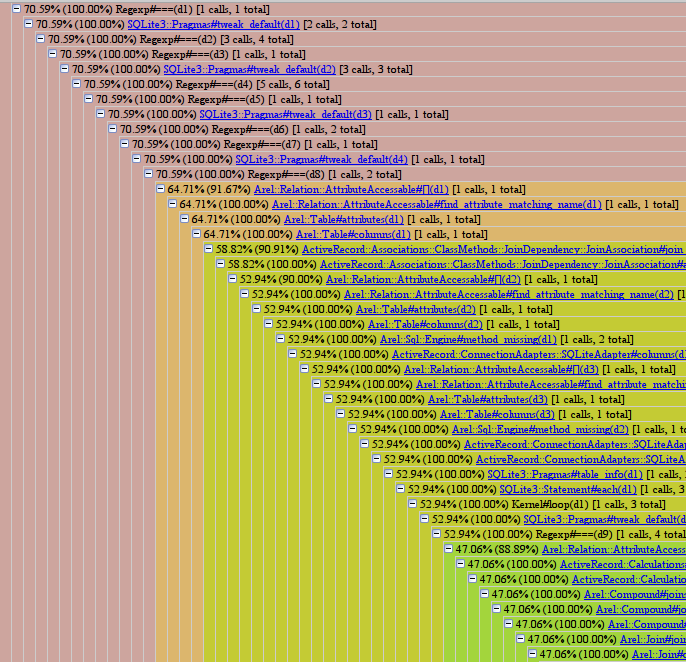
\includegraphics[width=0.9\textwidth]{ruby-prof_html_stack_printer}
  \caption{Ruby-prof HTML Stack Printer}
  \label{fig:ruby-prof_html_stack_printer}
\end{figure}
